\section{Применение средств автоматизированного проектирования \\
  при разработке устройства}

\subsection{Обоснование выбора пакетов прикладного программного обеспечения \\
  для моделирования и проектирования устройства}

Из-за приверженности к свободному программному обеспечению
~\cite{GNU-philosophy}, для создания проекта печатной платы была
выбрана САПР с открытым исходным кодом \textit{KiCAD}
~\cite{kicad-license}.

Такой выбор связан, этическими соображениями, которые, будучи
кратко сформулированы, звучат как:
Если пользователи не контролируют программу,
программа контролирует пользователей ~\cite{unfair-nonfree-programms}.

Для того, чтобы пользователи контролировали программу, требуется
четыре фундаментальные свободы~\cite{unfair-nonfree-programms}:

\begin{enumerate}
\item Свобода выполнять программу как вам угодно, в любых целях;
  
\item Свобода изучать “исходный текст” программы и править его, чтобы
программа проводила ваши вычисления как вам угодно. Программы пишутся
программистами на языках программирования (сочетающих естественные
языки с алгеброй) — и это образует форму программы, которую называют
“исходный текст”. Всякий, кто умеет программировать и у кого есть
программа в форме исходного текста, может прочесть исходный текст и
понять, как она работает, а также внести изменение. Когда все, что у
вас есть — это исполняемая форма, последовательность чисел, которые
компьютер эффективно выполняет, но которые человеку понимать крайне
трудно, то разбираться в программе и править ее в этом виде трудно до
невозможности.

\item  Свобода копировать и распространять свободные копии когда вам
угодно. (Это не обязанность; вы делаете это по своему выбору. Если
программа свободна, это не значит, что кто-то обязан предлагать вам
копию или что вы обязаны предлагать копию ему. Распространение
программы среди пользователей без свободы несправедливо по отношению к
ним; однако решение не распространять программу — пользоваться ею
частным порядком — не сопряжено с несправедливостью в отношении
кого-либо.)

\item Свобода копировать и распространять свои измененные версии когда
вам угодно.
\end{enumerate}

Другая причина выбора данной САПР при разработке,
используемый в ней, текстовой формат файлов,
при котором данные в документах САПР представлены
не иначе как Эс-Выражения (англ. \textit{S-Expressions})
~\cite{kicad-sexpr}.

В отличие от бинарных файлов,
используемых в \textit{Altium Designer},
файлы созданные при разработке печатной платы,
в \textit{KiCAD} за счёт их использования текста
возможно разместить в репозитории системы контроля версий
\textit{git}.

\textit{Git} это распределённая система контроля версий 
исходного кода \cite{git-dvcs}.

Из-за формата, файлы \textit{KiCAD} могут быть обработаны, как
исходный код.
Это даёт возможность удобной кооперации, при совместной работе.

Например в едином репозитории печатной платы, один конструктор в
соответствующем файле создаёт принципиальную схему устройства, а
другой в свою очередь, синхронизировав изменения в файле через
\textit{git}, используя готовую схему трассирует печатную плату.

Более того, используя, так называемый монорепозиторий, как подход
работы с \textit{git}, в одном репозитории можно содержать как
печатную плату, так и исходный код прошивки микроконтроллера,
используемый в ней.

\begin{figure}[H]
  \centering
  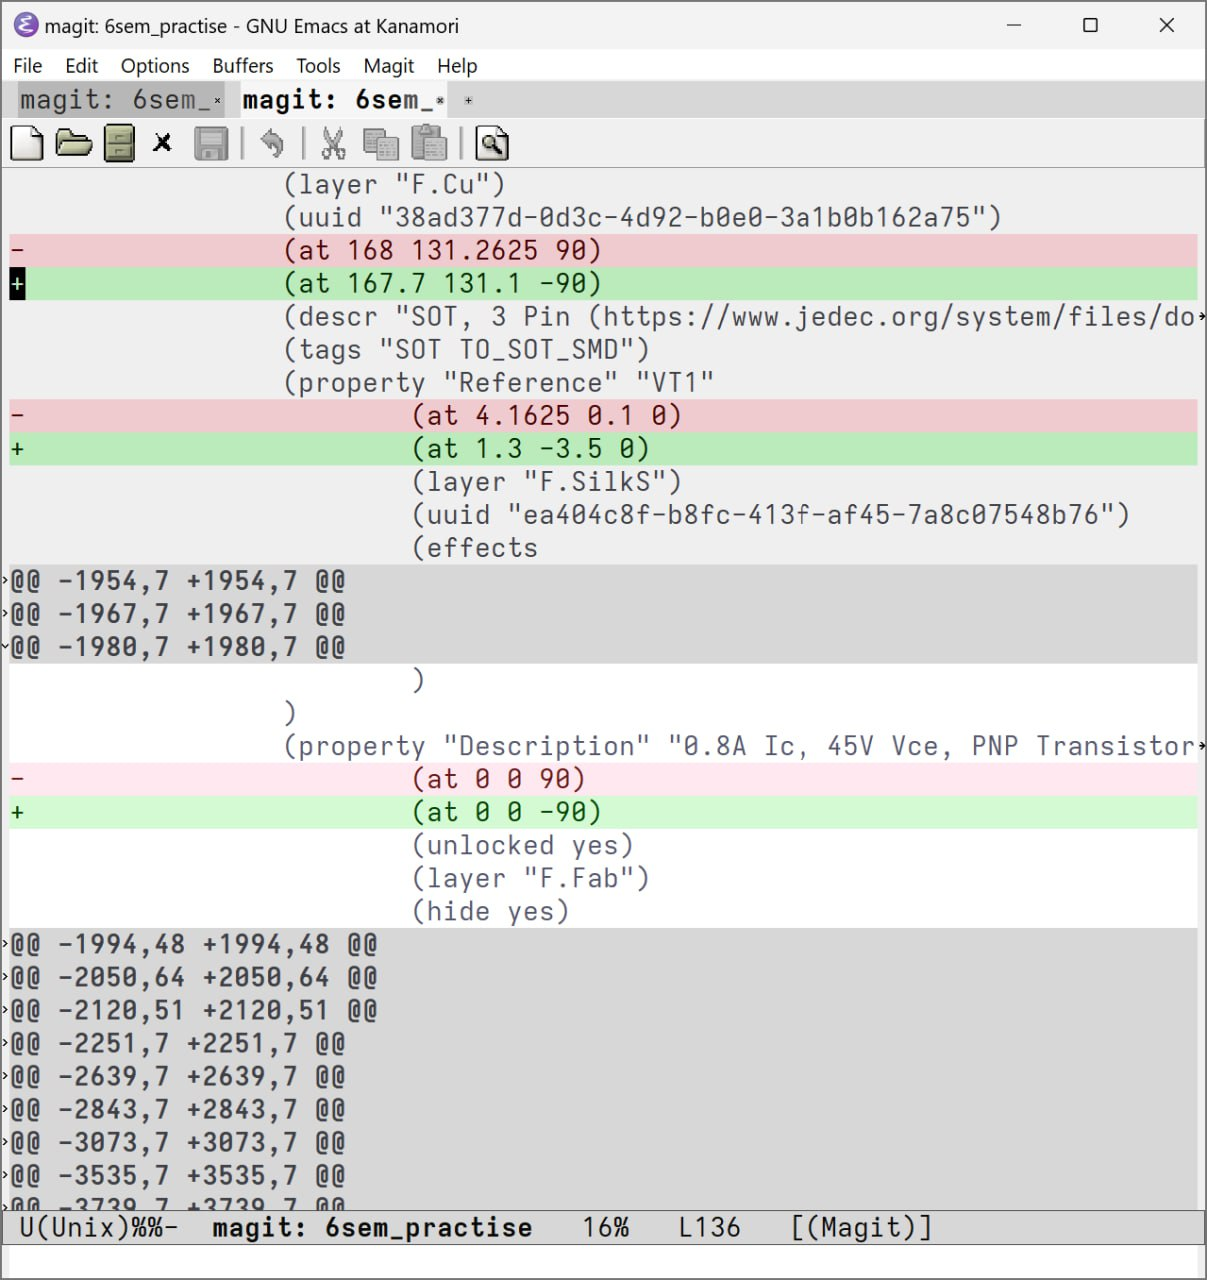
\includegraphics[scale=0.5]{magit-6-sem-practise.jpg}
  \caption{Снимок экрана с окном \textit{magit},
    установленный в расширяемый редактор текста \textit{GNU Emacs}
    клиент системы контроля версий \textit{git}.
    Видно, как \textit{magit} может распознать изменения файла трассировки печатной платы,
    как добавление и удаление строк.}
\end{figure}

Для разработки печатной платы данного электронного модуля было
достаточно использование САПР ПП \textit{KiCAD}, однако стоит
отметить, что использование специальных САПР симуляторов,
например \textit{Proteus} или \textit{SimulIDE}
позволяет промоеделировать работу прицнипальной схемы,
используемой в ПП, а также получить информацию
нужную, например для вычисления коээфицента нагрузки устройства
$K_{\textrm{Н}}$ при расчете надёжности.

Для моделирования корпуса печатной платы использовался
трёхмерный параметрический САПР \textit{Компас 3D}.
Данная программа была выбрана ввиду доступности
её учебной версии, а также широким возможностям,
позволяющим конкурировать с программами
занимающими передовые места на рынке
трехмерных параметрических САПР.

Логично было бы использовать открытый трёхмерный параметрический
САПР \textit{FreeCAD}, но на момент начала курсового проектирования,
данная программа ещё не достигла релизной версии и
проходила бета-тест~\cite{FreeCAD-Version-1-Released}.

Таким образом был достигнут компромисс между принципом использования
свободного программного обеспечения и требованиеям к выполнению чертежей.

\subsection{Технология применения средств автоматизированного проектирования \\
  при разработке конструкторской документации}

Большую сложность при выполнении работы составила необходимость
выполнять чертёж платы.
Интерфейс \textit{KiCAD-pcbdoc} рассчитан под трассировку печатной
платы, но никак не под черчение отдельного чертежа.
Присуствует возможность редактировать форматную рамку, наносить
разнообраные размеры, чертить на пользовательском слое.
Однако возможности выделить
каждый слой платы как отдельный вид на чертеже нет.

\textit{CALS (continuous acquisition and lifecycle support) } — это
непрерывная информационная поддержка жизненного цикла продукта.
Внедрение \textit{CALS}-технлогий на предприятии обычно
предполагает~\cite{Lanin2019}:
\begin{enumerate}
\item Полное реформирование процессов на предприятии, включая
проектирование, конструирование, подготовку, производства, закупки,
производство, управление, материално-техническое снабжение, сервисное
обслуживание;

\item Использование современных информационных технологий;
  
\item Совместное использование данных, полученных на различных стадиях
  жизненного цикла продукта;
  
\item Применение международных стандартов в области информационных
технологий в целях интеграции, совместного использования информации и
упралвения ею.
\end{enumerate}

Были внедредны следующие CALS-технологии:
\begin{enumerate}
\item Файлы \textit{STEP} для экспорта трехмерной модели печатной
платы, которая использовалась для того, чтобы разработать корпус
платы.

\item Файлы \textit{DXF} использовались для экспорта отдельных слоев
печатной платы, для создания чертежа печатной платы.
\end{enumerate}

Для выполнения поставленных задач, были использован максимум
возможностей предоставляемых выбранными САПР.

\newpage
%%% Local Variables:
%%% mode: LaTeX
%%% TeX-master: "main"
%%% End:
